% !TEX encoding   = UTF8
% !TEX spellcheck = ru_RU
% !TEX root = ../seminars.tex

%%=================================
\section{Правильные многоугольники}
%%=================================
Нарисуем ряд вложенных правильных многоугольников из~упражнения~11 \textbookref{главы~12}.

\begin{figure}[ht]
  {\centering
    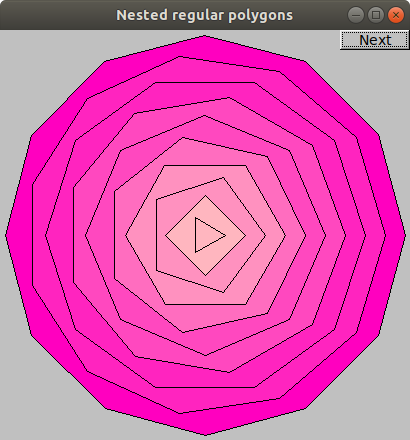
\includegraphics[height=0.3\textwidth]{images/regular_polygons.png}

  }
  \caption{Вложенные правильные многоугольники}
  \label{fig:regpoly}
\end{figure}

Покажем лишь ключевой фрагмент кода. Напомним, что функция \code{regular\_polygon()} вычисляет вершины правильного многоугольника и была представлена ранее в~разделе~\ref{sect:geomelems}.

\cppfile[firstline=19, lastline=45]{projects/11/regular_polygons.cpp}

Класс \code{Vector\_ref} рассматривается в~\textbookref{главе~13} и удобен для~хранения множества неименованных объектов. Многоугольники рисуются с~использованием вращательной симметрии и раскрашиваются в~оттенки пурпурного (см. диаграмму цветов из~\textbookref{главы~13}). Результат работы программы показан на~рисунке~\ref{fig:regpoly}.



%%====================
\section{Суперэллипсы}
%%====================
Суперэллипс, также известный как кривая Лямэ, названная в~честь \href{https://en.wikipedia.org/wiki/Gabriel_Lam\%C3\%A9}{Габриэля Лямэ}, "--- замкнутая кривая, которая как и эллипс обладает большой и малой полуосями, а также симметрией относительно них, но в~общем случае другой формой.

\begin{figure}[ht]
  {\centering
    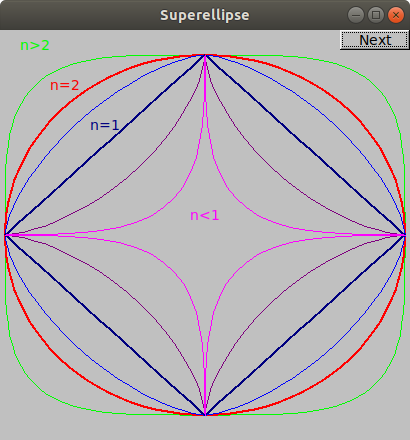
\includegraphics[height=0.3\textwidth]{images/superellipse.png}

  }
  \caption{Суперэллипсы}
  \label{fig:superellipse}
\end{figure}

В~декартовой системе координат суперэллипс в~обобщённом виде задаётся следующим соотношением:
\[
  \left| \frac{x}{a} \right|^m + \left| \frac{y}{b} \right|^n = 1;\quad m, n > 0.
\]

В~параметрическом виде, где параметр~\(t\) не~имеет никакой геометрической интерпретации, кривая выражается системой уравнений:
\begin{equation}
  \label{eq:superellipse}
  \left\{\begin{array}{l}
    x(t) = a\,\mathrm{sign}(\cos t) \cdot |\cos t|^{\frac{2}{m}},\\
    y(t) = b\,\mathrm{sign}(\sin t) \cdot |\sin t|^{\frac{2}{n}};
  \end{array}\right.
  \quad 0 \leqslant t \leqslant 2\pi.
\end{equation}

Функция, добавляющая точки, лежащие на~суперэллипсе, по~формуле~(\ref{eq:superellipse}), приведена ниже:

\cppfile[firstline=20, lastline=35]{projects/11/superellipse.cpp}

Функцию, определяющую знак числа, можно написать таким образом:

\cppfile[firstline=18, lastline=18]{projects/11/superellipse.cpp}

Ключевой фрагмент функции \code{main()} для~рисования нескольких вложенных суперэллипсов из~упражнения~12 \textbookref{главы~12}:

\cppfile[firstline=40, lastline=54]{projects/11/superellipse.cpp}

Мы уверены, что вы сможете самостоятельно добавить текстовые метки (подписи) к~кривым и раскрасить их, например, как на~рисунке~\ref{fig:superellipse}.
